% Matlab 画图
% Matlab|编程|画图

\pentry{Matlab 的函数\upref{MatFun}}

Matlab 具有强大的画图功能, 这里仅介绍一些基础知识. 最常用的画图函数是 \lstinline|plot|, 例如
\begin{lstlisting}[language=MatlabCom]
>> x = linspace(0, 2*pi, 100); y = sin(x);
>> plot(x, y);
\end{lstlisting}
结果如\autoref{MatPlt_fig1}(左) 所示. 如果要在该坐标系继续画图, 要用 \lstinline|hold on| 命令(\lstinline|on| 是 \lstinline|hold| 的输入变量), 否则每用一次 \lstinline|plot|, 之前画过的图都会被清除. 用 \lstinline|hold off| 可以重新恢复自动清除.
\begin{lstlisting}[language=MatlabCom]
>> y1 = cos(x);
>> hold on; plot(x, y1);
\end{lstlisting}
结果如\autoref{MatPlt_fig1}(右) 所示, 注意新增曲线的颜色变化.
\begin{figure}[ht]
\centering
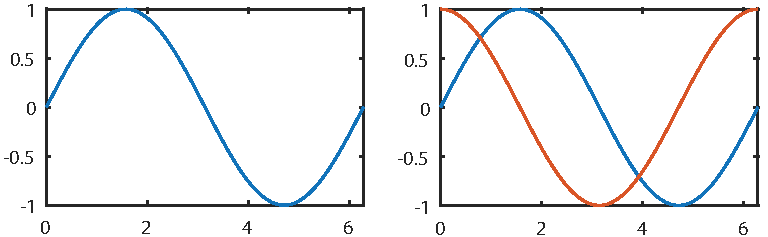
\includegraphics[width=13cm]{./figures/MatPlt1.pdf}
\caption{\lstinline|plot| 函数} \label{MatPlt_fig1}
\end{figure}

如果我们要新建一个画图窗口, 用 \lstinline|figure| 函数. 若要指定画图的颜色, 可以添加 \lstinline|figure| 的第三个变量, 用一个字符表示颜色(red:\lstinline|'r'|, green:\lstinline|'g'|, blue:\lstinline|'b'|, yellow:\lstinline|'y'|, magenta: \lstinline|'m'|, cyan: \lstinline|'c'|, black: \lstinline|'k'|, white: \lstinline|'w'|). 例如
\begin{lstlisting}[language=MatlabCom]
>> x2 = cos(x); y2 = sin(x);
>> figure; plot(x2, y2, 'r');
\end{lstlisting}
在新增的窗口中, 结果如\autoref{MatPlt_fig2} (左)所示. 注意根据窗口尺寸的不同, $x$ 轴和 $y$ 轴的单位长度一般不同, 若要使其相同, 可以在 \lstinline|plot| 后面用 \lstinline|axis equal| 命令(其中字符串 \lstinline|equal| 是 \lstinline|axis| 函数的输入变量), 得到\autoref{MatPlt_fig2} (右).
\begin{figure}[ht]
\centering
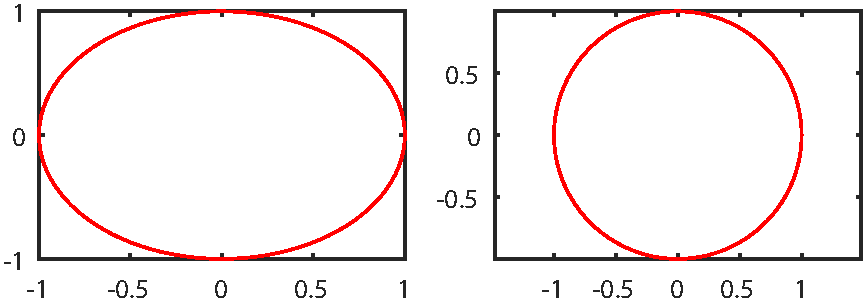
\includegraphics[width=13cm]{./figures/MatPlt2.pdf}
\caption{红色的单位圆} \label{MatPlt_fig2}
\end{figure}
若要调整坐标轴的范围, 也可用 \lstinline|axis| 函数. 另外可以在 \lstinline|plot| 的第三个变量的字符串中设定曲线的形状, 用 \lstinline|xlabel| 和 \lstinline|ylabel| 函数分别设置 $x$ 轴和 $y$ 轴的文字, 用 \lstinline|title| 函数设置图片标题
\begin{lstlisting}[language=MatlabCom]
>> plot(x2, y2, '.-r');
>> axis([-1.2, 1.2, -1.2, 1.2]);
>> xlabel('x'); ylabel('y'); title('unit circle');
\end{lstlisting}
其中 \lstinline|'.-'| 表示带点的连线,点的坐标由 \lstinline|x2| 和 \lstinline|y2| 决定(另外 \lstinline|'+-'| 表示带加号的连线, \lstinline|'o-'| 表示带圆圈的连线). \lstinline|axis| 中行矢量中的四个数分别是 $x$ 轴的最小最大值和 $y$ 轴的最小最大值. 结果如\autoref{MatPlt_fig3} (左)所示.
\begin{figure}[ht]
\centering
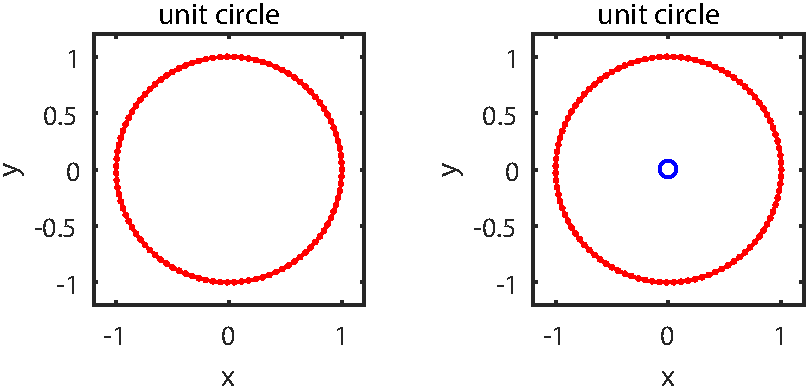
\includegraphics[width=11cm]{./figures/MatPlt3.pdf}
\caption{红色的单位圆} \label{MatPlt_fig3}
\end{figure}

除了 \lstinline|plot| 以外, 常用的还有 \lstinline|scatter| 函数, 用于画散点图. 格式与 \lstinline|plot| 相似. 默认的散点形状是圆圈, 但也可以在第三个变量中设置颜色和 \lstinline|'+'|, \lstinline|'x'|, \lstinline|'.'| 等形状. 例如
\begin{lstlisting}[language=MatlabCom]
>> hold on; scatter(0, 0, 'b');
\end{lstlisting}
结果如\autoref{MatPlt_fig3} (右)所示.

最后, 如果要关闭当前画图窗口, 用 \lstinline|close| 函数(无输入变量), 如果要关闭所有窗口, 用 \lstinline|close all| 即可.
